
%%%%%%%%%%%%%%%%%%%%%%%%%%%%%%%%%%%%%%%%
\documentclass{paper}
%%%%%%%%%%%%%%%%%%%%%%%%%%%%%%%%%%%%%%%%


\ifx\pdftexversion\undefined
    \usepackage[dvips]{graphicx}
\else
    \usepackage[pdftex]{graphicx}
    \usepackage{epstopdf}
    \epstopdfsetup{suffix=}
\fi



%%%%%%%%%%%%%%%%%%%%%%%%%%%%%%%%%%%%%%%%
\begin{document}
%%%%%%%%%%%%%%%%%%%%%%%%%%%%%%%%%%%%%%%%


\section{Data}

Summary statistics for numerical variables are shown in Table \ref{tab:summary}. 

% latex table generated in R 4.0.2 by xtable 1.8-4 package
% Sat Oct 17 21:18:35 2020
\begin{table}[ht]
\centering
\begin{tabular}{rlrr}
  \hline
 & Statistic & house\_price & income \\ 
  \hline
1 & Min. & 0.19 & 0.08 \\ 
  2 & Mean & 0.70 & 0.10 \\ 
  3 & S.D. & 0.18 & 0.01 \\ 
  4 & Max. & 1.09 & 0.13 \\ 
   \hline
\end{tabular}
\caption{Summary of Numeric Variables} 
\label{tab:summary}
\end{table}



Table \ref{tab:earthquakes} shows the frequency of observations in and out of California along with the incidence of earthquakes. Notice that earthquakes have only happened in California. 

% latex table generated in R 4.0.2 by xtable 1.8-4 package
% Thu Oct 22 10:50:50 2020
\begin{table}[ht]
\centering
\begin{tabular}{rrr}
  \hline
 & None & Earthquake \\ 
  \hline
Other &  50 &   0 \\ 
  California &  46 &   4 \\ 
   \hline
\end{tabular}
\caption{Earthquake Incidence by State} 
\label{tab:earthquakes}
\end{table}


The correlation matrix of potential variables in the model is shown in Table \ref{tab:corr}. 
House prices are positively correlated with income and California but negatively correlated with earthquakes. In the next setion, these variables will be included in a regression model. 

\input{../Tables/correlation.tex}



\pagebreak
\section{Empirical Results}


\begin{figure}
\centering
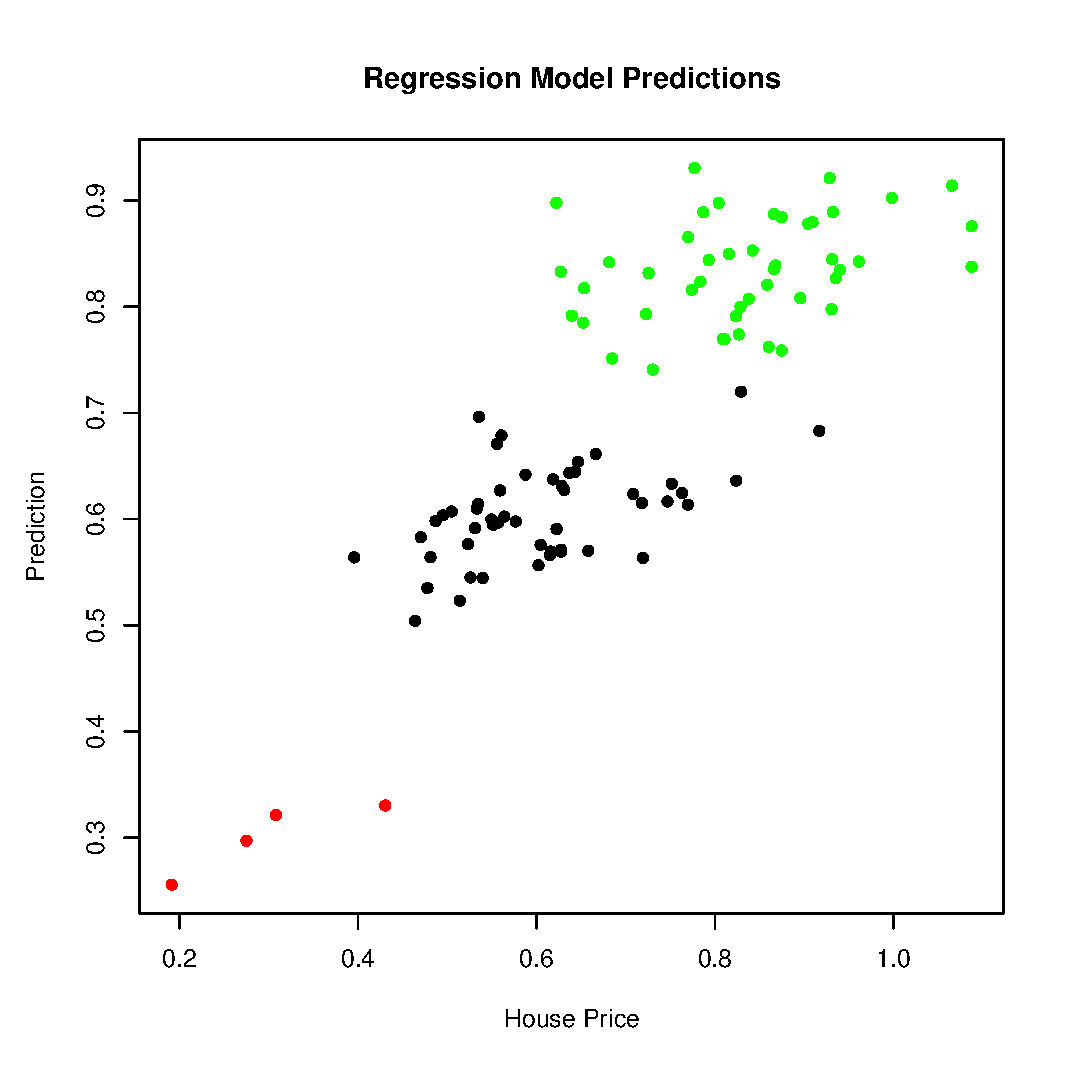
\includegraphics[width=\textwidth]{../Figures/predictions.eps}
\caption{House Prices vs. Predicted Prices}
\label{fig:pred}
\end{figure}


The regression lines are shown in Figure \ref{fig:reg}, with the estimated intercept term for zip codes affected by earthquakes (red), those in the rest of California (green), and the zip codes outside of California. 

\begin{figure}
\centering
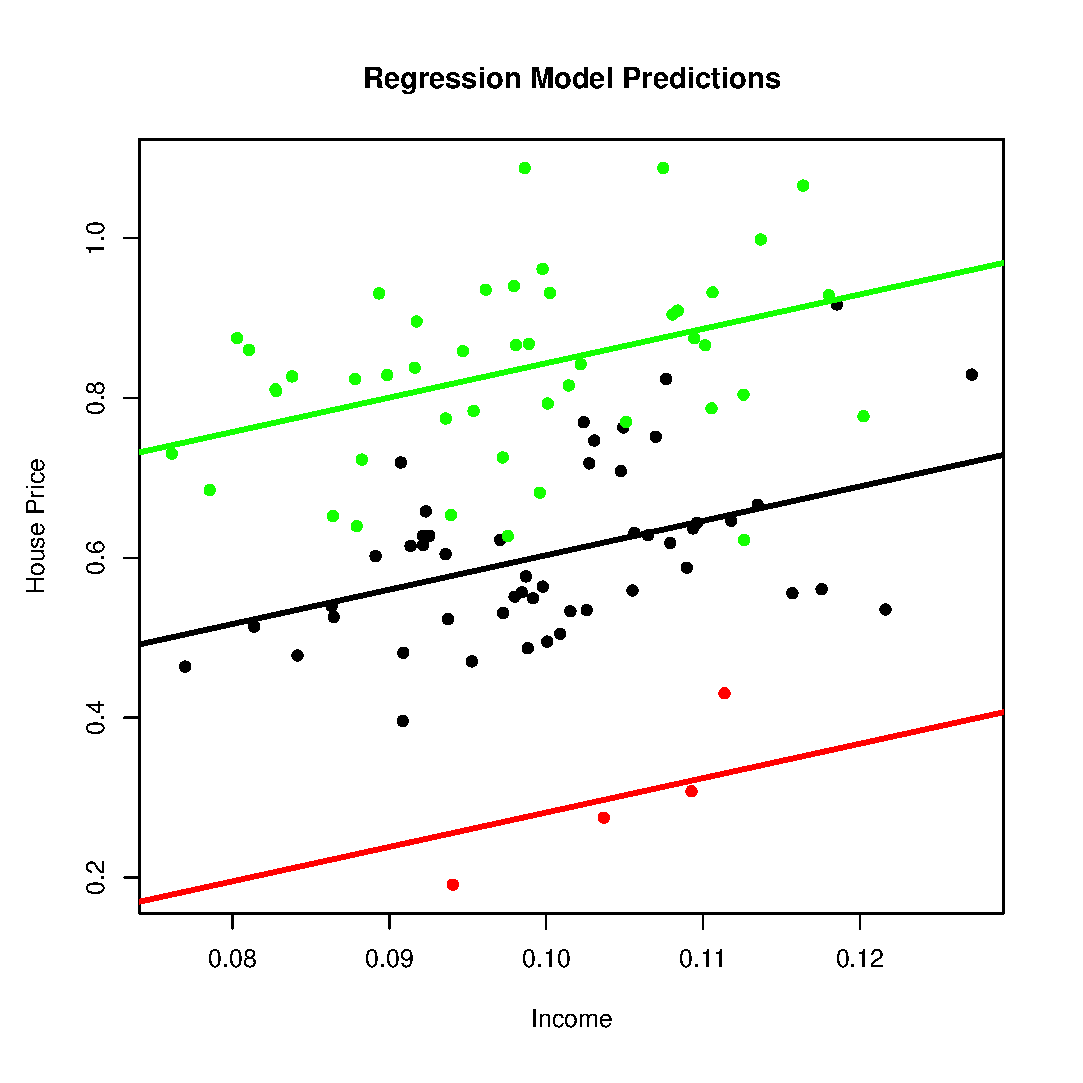
\includegraphics[width=\textwidth]{../Figures/regression.eps}
\caption{Regression Model Predictions}
\label{fig:reg}
\end{figure}





%%%%%%%%%%%%%%%%%%%%%%%%%%%%%%%%%%%%%%%%
\end{document}
%%%%%%%%%%%%%%%%%%%%%%%%%%%%%%%%%%%%%%%%